
%\documentclass[conference]{IEEEtran}
\documentclass[10pt,conference]{IEEEtran}

\pagestyle{plain}

\usepackage[english,american]{babel}
\usepackage{graphicx}
\usepackage{subfigure}
\usepackage{amsmath}
\usepackage{multirow}
\usepackage{multicol}
\usepackage{float}
\usepackage{algorithm}
\usepackage{algorithmic}
\usepackage[colorlinks, linkcolor=red, anchorcolor=green, citecolor=blue]{hyperref}
\usepackage{cite}
\usepackage{balance}
\usepackage{color}
\usepackage[square,sort,comma,numbers]{natbib}
\usepackage{url}
\usepackage{diagbox}
\usepackage{enumerate}
\usepackage{setspace}
\let\labelindent\relax
\usepackage{enumitem}
\usepackage{indentfirst}
\usepackage{booktabs}
\usepackage{tikz}
\usepackage{listings}
\usepackage{etoolbox}
\usepackage{setspace}

\hyphenation{op-tical net-works semi-conduc-tor}
%\renewcommand{\baselinestretch}{0.985}
%\renewcommand{\captionfont}{\linespread{1.5}\normalsize}

%\renewcommand{\thesection}{\arabic{section}}
%\renewcommand{\thesubsection}{\thesection.\arabic{subsection}}
%\renewcommand{\thesubsubsection}{\thesubsection.\arabic{subsubsection}}

%\makeatletter
%\def\@seccntformat#1{\@ifundefined{#1@cntformat}%
%   {\csname the#1\endcsname\quad}%       default
%   {\csname #1@cntformat\endcsname}}%    enable individual control
%\newcommand\section@cntformat{}
%\makeatother

\renewcommand{\algorithmicrequire}{\textbf{Input:}}
\renewcommand{\algorithmicensure}{\textbf{Output:}}
%\usepackage{setspace}
%\usepackage{epsfig,graphics,subfigure,psfrag,amsmath,amssymb}
\newcommand\FIXME[1]{\textcolor{red}{FIX:}\textcolor{red}{#1}}
\newcommand\FIXED[1]{\textcolor{blue}{FIXED: }\textcolor{blue}{#1}}

%\def\@IEEEsectpunct{.\ \,}
%\def\paragraph{\@startsection{paragraph}{4}{\z@}{1.5ex plus 1.5ex minus 0.5ex}%
%{0ex}{\normalfont\normalsize\sffamily\bfseries}}


\newcommand{\circled}[2][]{\tikz[baseline=(char.base)]
    {\node[shape = circle, draw, inner sep = 1pt]
    (char) {\phantom{\ifblank{#1}{#2}{#1}}};%
    \node at (char.center) {\makebox[0pt][c]{#2}};}}
\robustify{\circled}

\begin{document}
%\setcopyright{acmcopyright}

\title{Using Facial Behavior Biometric Modalities for Smartphone Authentication}
\author{
%\IEEEauthorblockN{Guixin Ye\IEEEauthorrefmark{2},
%Zhanyong Tang$^{*,}$\IEEEauthorrefmark{2}\thanks{*Corresponding authors: Zhanyong Tang and Zheng Wang},
%Dingyi Fang\IEEEauthorrefmark{2},
%Xiaojiang Chen\IEEEauthorrefmark{2},
%Kwang In Kim\IEEEauthorrefmark{3},
%Ben Taylor\IEEEauthorrefmark{4}, and
%Zheng Wang$^{*,}$\IEEEauthorrefmark{4}}
%\IEEEauthorblockA{\IEEEauthorrefmark{2}School of Information Science and Technology, Northwest University, China\\Email:  gxye@stumail.nwu.edu.cn, \{zytang, dyf, xjchen\}@nwu.edu.cn}
%\IEEEauthorblockA{\IEEEauthorrefmark{3}Department of Computer Science, University of Bath, UK\\Email: k.kim@bath.ac.uk}
%\IEEEauthorblockA{\IEEEauthorrefmark{4}School of Computing and Communications, Lancaster University, UK\\Email: \{b.d.taylor, z.wang\}@lancaster.ac.uk}
}

\IEEEoverridecommandlockouts
\makeatletter\def\@IEEEpubidpullup{9\baselineskip}\makeatother
\IEEEpubid{\parbox{\columnwidth}{Permission to freely reproduce all or part
    of this paper for noncommercial purposes is granted provided that
    copies bear this notice and the full citation on the first
    page. Reproduction for commercial purposes is strictly prohibited
    without the prior written consent of the Internet Society, the
    first-named author (for reproduction of an entire paper only), and
    the author's employer if the paper was prepared within the scope
    of employment.  \\
    NDSS '17, 26 February -1 March 2017, San Diego, CA, USA\\
    Copyright 2017 Internet Society, ISBN 1-891562-41-X\\
    http://dx.doi.org/10.14722/ndss.2017.23xxx
}
\hspace{\columnsep}\makebox[\columnwidth]{}}

\maketitle

\begin{abstract}

Pattern lock is widely used as a mechanism for authentication and authorization on Android devices. This paper presents a novel video-based attack to reconstruct Android lock patterns from video footage filmed using a mobile phone camera. Unlike prior attacks on pattern lock, our approach does not require the video to capture any content displayed on the screen. Instead, we employ a computer vision algorithm to track the fingertip movements to infer the pattern. Using the geometry information extracted from the tracked fingertip motions, our approach is able to accurately identify a small number of
(often one) candidate patterns to be tested by an adversary.
We  thoroughly evaluated our approach using 120 unique patterns collected from 215 independent users, by applying it to reconstruct patterns from video footage filmed using smartphone cameras. Experimental results show that our approach can break over 95\% of the patterns in five attempts before the device is automatically locked by the Android operating system. We discovered that, in contrast to many people's belief, complex patterns do not offer stronger protection under our attacking scenarios. This is demonstrated by the fact that we are able to break all but one complex patterns
as opposed to  60\% of the simple patterns in the first attempt. Since our threat model is common in
day-to-day life, this paper calls for the community to revisit the risks of using Android pattern lock to protect sensitive information.
\\
\end{abstract}


%\begin{CCSXML}
%<ccs2012>
%<concept>
%<concept_id>10002978.10002991.10002992.10011618</concept_id>
%<concept_desc>Security and privacy~Graphical / visual passwords</concept_desc>
%<concept_significance>500</concept_significance>
%</concept>
%<concept>
%<concept_id>10002978.10003014.10003017</concept_id>
%<concept_desc>Security and privacy~Mobile and wireless security</concept_desc>
%<concept_significance>300</concept_significance>
%</concept>
%</ccs2012>
%\end{CCSXML}
%
%\ccsdesc[500]{Security and privacy~Graphical / visual passwords}
%\ccsdesc[300]{Security and privacy~Mobile and wireless security}
%
%\printccsdesc
% no keywords
%\keywords{Side-channel Attack, Android Pattern Lock, Authentication, Motion Tracking, Vision Analysis}\\

%TODO:
% Read: A pilot study on the security of pattern screen-lock methods and soft side channel attacks
\section{Introduction}

A CAPTCHA (Completely Automated Public Turing Test to Tell Computers and Human Apart) is a automated test that humans can pass but computer programs cannot~\cite{Von2004Telling}. It provides a effective approach for automatically distinguishing humans from computer systems, and therefore is used to defend against automatic spam, registration or malicious bots~\cite{Von2003CAPTCHA,Tam2008Breaking}.

The most widely deployed CAPTCHA is the so-called text-based scheme~\cite{Yan2008Usability}, which mainly consists of distorted English letters and Arabic numerals. The popularity of this scheme is due to its obvious advantages~\cite{Chellapilla2005Building,Chellapilla2005Computers}: (1) most people around the world can recognize English letters and Arabic numerals; (2) the space of the text-based Captcha are huge so that the brute-force attack can be defeated. Given its pervasive usage, a security breach of the text-based Captcha could lead to serious consequences.

The robustness of text-based Captchas is the significant concern in the research communities. Over the past decade, researchers have uncovered a number of ways to recognize text-based Captchas. Many fine prior researches just focus on attacking an unique Captcha scheme~\cite{Gao2013The,Gao2017Research,Mohamed2014A,Yan2008A}. This limits their applicability. Recently the generic attacks have been proposed by Gao \emph{et al.}~\cite{Gao2016A} and Bursztein \emph{et al.} ~\cite{Bursztein2011Text,Bursztein2014The}. They claim that they can break a wide range of text-based Captchas using a generic method. However, these defeated Captchas possess relative simple noisy background or uniform style. Although the security of text-based Captchas have been proven frail, many companies such as Google, Microsoft and Baidu still use such scheme as current text-based Captcha scheme have more complex background or distorted characters. This makes previous attacks invalid.  Recent studies~\cite{Thomas2013Trafficking,Bursztein2014Easy} also demonstrate that text-based Captcha is still a secure mechanism.

The key factor of previous attacks on text-based Captcha lies in the difficulty of segmenting characters~\cite{Chellapilla2005Computers}. Therefore, the basic design principle of text-based Captchas should be anti-segmentation. To this end, current text-based Captchas with more complex noisy background and distorted characters have been proposed and deployed by many companies. In order to increase the difficulty of finding where each character is, such Captcha shorten the distance between characters. All attacks proposed above were invalid due to cannot successfully segment the characters. It is therefore driving us wondering: is current Captcha scheme as secure as it is expected? This fundamental question precipitated our study.

In this paper, we present a novel generic attack on current text-based Captchas using deep learning technology. Our attack employs a variant of the generative adversarial network (GAN)~\cite{pix2pix2016} to transform the distorted captchas to the regular ones. The former serval layers of the GAN is used to remove the complicated noisy background. The middle layers aim to enlarge the distance between adjacent characters and output the distorted captchas with larger inter-character distance which are translated to regular ones by the last layers. At last, the transformed regular captchas are recognized by a Convolutional Neural Network (CNN).

We thoroughly evaluate our approach using real-world captchas collected from some websites. We show that our approach is effective in recognize current text-based captchas and as a results, we can defeat almost all current text-based captchas with a success rate range from XX\% to XX\%. We demonstrate that, the sophisticated noisy background cannot offer stronger protection in term of anti-segmentation under our attack. Our finding suggests that text-based captchas are insecure under the age of artificial intelligence.

        \begin{figure*}[!t]
            \centering
            \subfigure{
                \begin{minipage}[t]{0.2\textwidth}
                    
\includegraphics[width=\textwidth]{fig/prior_captcha11.png}\\
                    \center (a) Character isolated Captcha
                \end{minipage}
            }
            \hspace{0.16cm}
            \subfigure{
                \begin{minipage}[t]{0.20\textwidth}
                    
\includegraphics[width=\textwidth]{fig/prior_captcha2.png}\\
                    \center (b) Megaupload
                \end{minipage}
            }
            \hspace{0.16cm}
            \subfigure{
                \begin{minipage}[t]{0.20\textwidth}
                    
\includegraphics[width=\textwidth]{fig/prior_captcha3.png}\\
                    \center (c) Yahoo!
                \end{minipage}
            }
            \hspace{0.16cm}
            \subfigure{
                \begin{minipage}[t]{0.20\textwidth}
                    
\includegraphics[width=\textwidth]{fig/prior_captcha4.png}\\
                    \center (d) Recaptchas
                \end{minipage}
            }
            \hspace{0.16cm}
            \subfigure{
                \begin{minipage}[t]{0.20\textwidth}
                    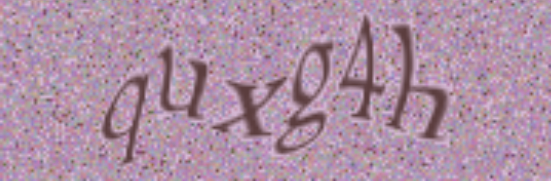
\includegraphics[width=\textwidth]{fig/prior_captcha7.png} \\
                    \center (e) Skyrock
                \end{minipage}
            }
            \hspace{0.16cm}
            \subfigure{
                \begin{minipage}[t]{0.20\textwidth}
                    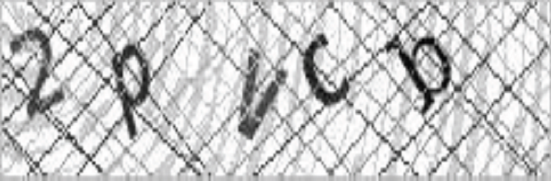
\includegraphics[width=\textwidth]{fig/prior_captcha8.png} \\
                    \center (f) Digg
                \end{minipage}
            }
            \hspace{0.16cm}
            \subfigure{
                \begin{minipage}[t]{0.20\textwidth}
                    
\includegraphics[width=\textwidth]{fig/prior_captcha9.png}\\
                    \center (g) Reddit
                \end{minipage}
            }
            \hspace{0.16cm}
            \subfigure{
                \begin{minipage}[t]{0.20\textwidth}
                    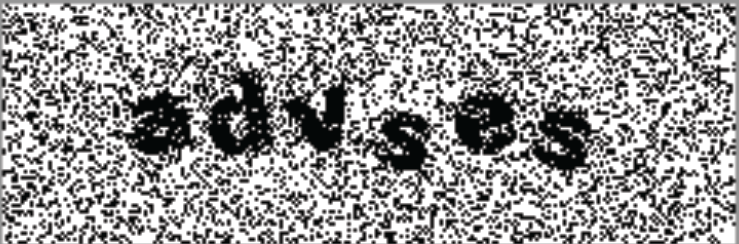
\includegraphics[width=\textwidth]{fig/prior_captcha10.png}\\
                    \center (h) Captcha.net
                \end{minipage}
            }
            \subfigure{
                \begin{minipage}[t]{\textwidth}
                    \center (1) Captchas used in previous attacks.\\
                \end{minipage}
            }
            \hspace{0.16cm}
            \subfigure{
                \begin{minipage}[t]{0.20\textwidth}
                    
\includegraphics[width=\textwidth]{fig/prior_captcha11.jpg} \\
                    \center (i) Tecent
                \end{minipage}
            }
            \hspace{0.16cm}
            \subfigure{
                \begin{minipage}[t]{0.20\textwidth}
                    
\includegraphics[width=\textwidth]{fig/prior_captcha12.jpg} \\
                    \center (j) Baidu
                \end{minipage}
            }
            \hspace{0.16cm}
            \subfigure{
                \begin{minipage}[t]{0.20\textwidth}
                    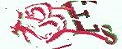
\includegraphics[width=\textwidth]{fig/prior_captcha13.jpg}\\
                    \center (k) NetEase
                \end{minipage}
            }
            \hspace{0.16cm}
            \subfigure{
                \begin{minipage}[t]{0.20\textwidth}
                    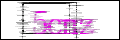
\includegraphics[width=\textwidth]{fig/prior_captcha14.jpg}\\
                    \center (l) VIPSHOP
                \end{minipage}
            }
            \subfigure{
                \begin{minipage}[t]{\textwidth}
                    \center (2) Current Captchas deployed in some popular websites.\\
                \end{minipage}
            }
            \caption{This shows the text-based Captcha schemes used in prior works and current Captchas deployed in some famous websites. The scheme in (a) shows the character isolated Captcha that is deployed originally.}
            \label{fig:text-based captchas}
        \end{figure*}

\textbf{Contributions} This paper makes the following specific contributions:

In order to design a more security Captcha scheme, currently Captchas deployed by many companies 
%\begin{figure*}[!t]
  \centering
  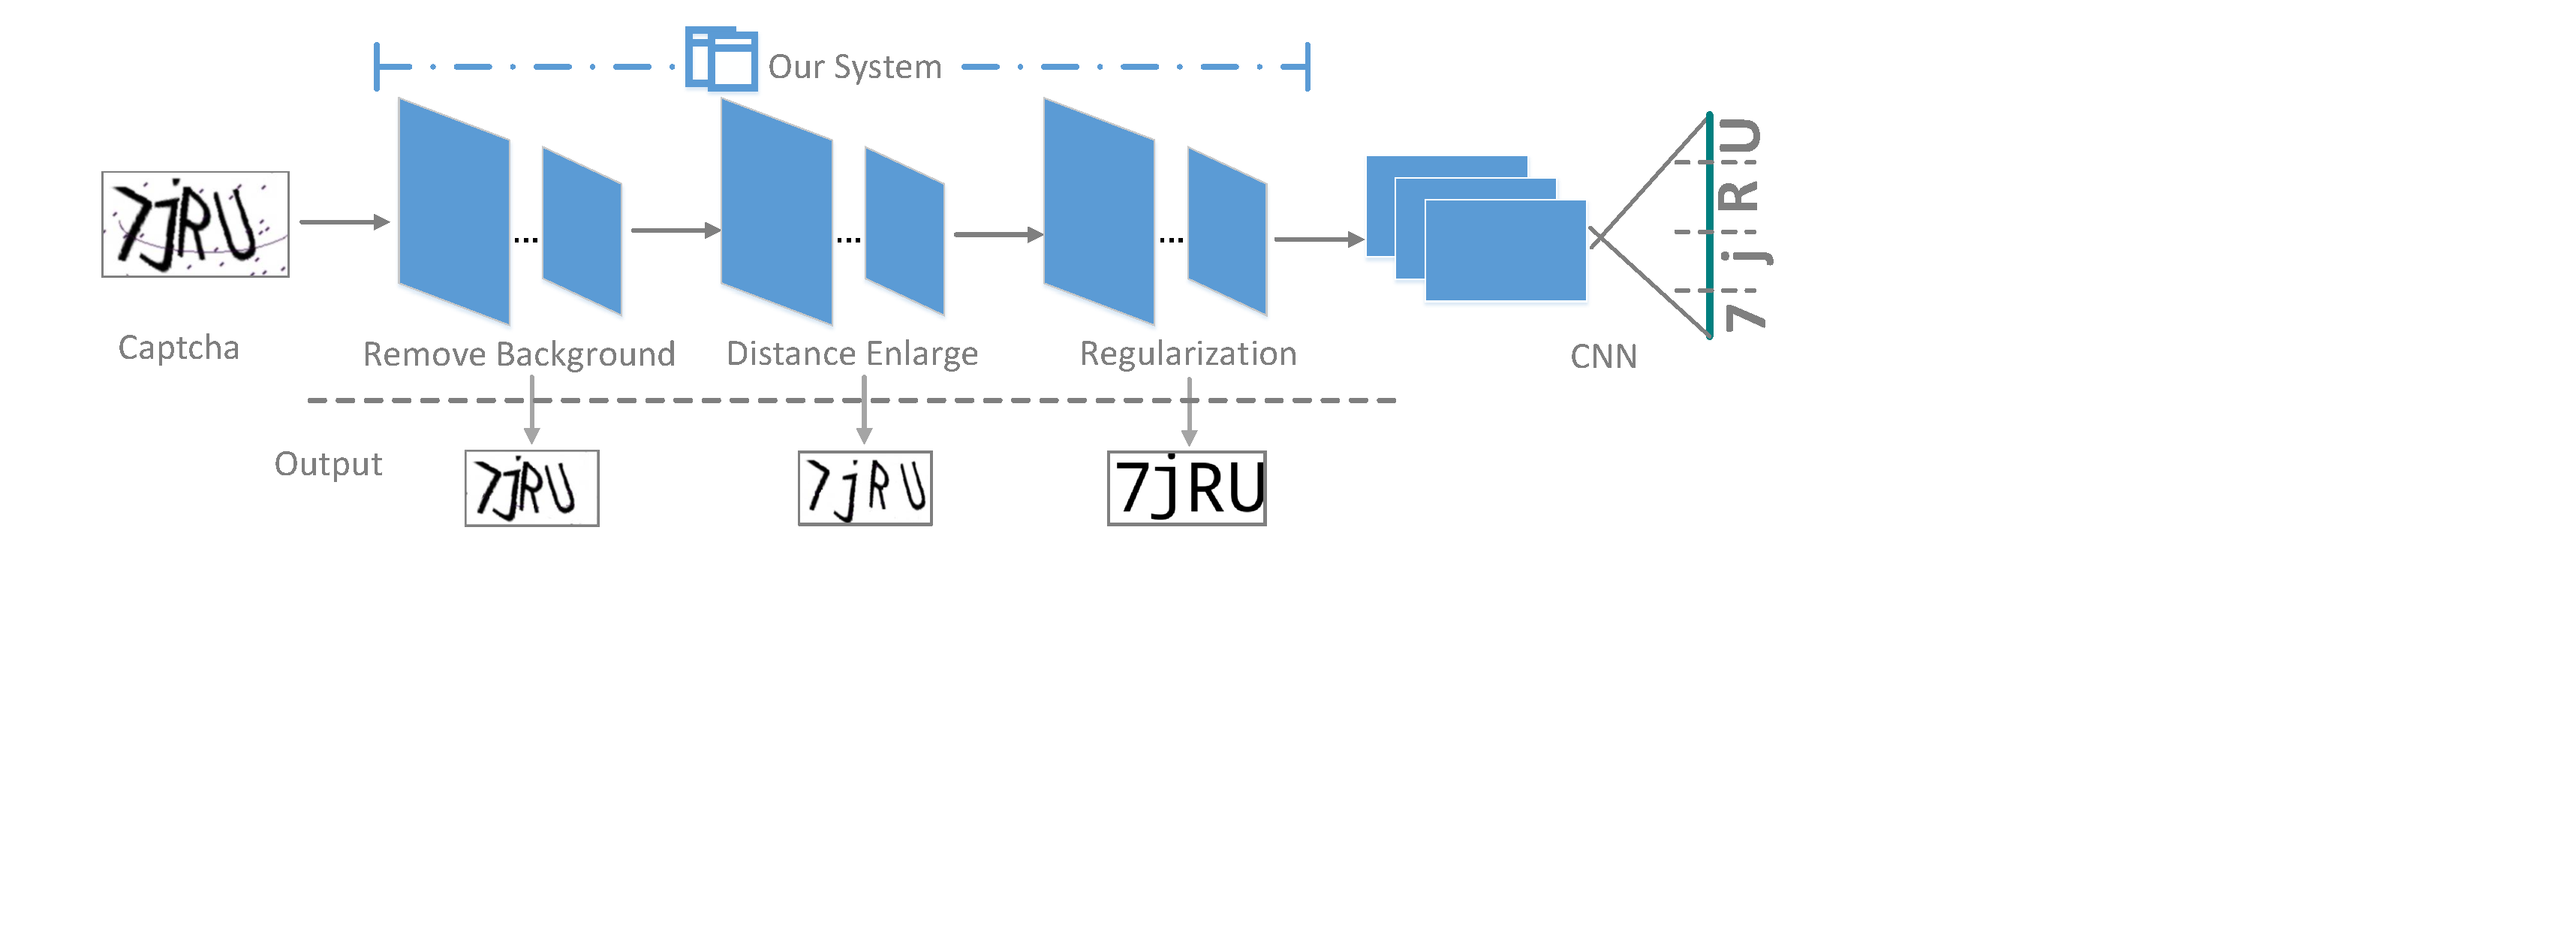
\includegraphics[width=0.9\textwidth]{fig/overview.pdf}
  \caption{The overview of our attack.}
  \label{fig:overview}
\end{figure*}

\section{Background}

\subsection{Text-based Captchas}

CAPTCHA is also called inverse Turing test~\cite{Naor1996Verification}, and aims to determine whether or not the user is human. The most popularity of Captchas is text-based Captchas. Initially, they were composed of deformed English letters and Arabic numerals which human can recognize while computers cannot. The usage of English letters and Arabic numerals makes text-based Captchas being welcomed world-wide~\cite{Chellapilla2005Building,Chellapilla2005Computers}. Due to such advantages, text-bsaed Captchas have been widely used in various of Internet security access tasks~\cite{Von2004Telling}. These tasks include defending against malicious scraping web contents, preventing automatic registration of free accounts for spam posting or forums, or mitigating the impact of DDoS attacks.

\subsubsection{Captcha Security Features} \label{section: sccturity_features}
To summary out a representative security features, we collected a wide range of Captchas that had ever been or being used by the top 20 most popular web sites which are listed by Alexa~\footnote{http://www.alexa.com/topsites}. Figure~\ref{fig:text-based captchas} gives some representative examples of our collected Captchas~\footnote{Some previous used Captchas come from the related works~\cite{Gao2013The,Gao2016A,Bursztein2011Text}.}. It obviously shows that current text-based Captchas have more complex security features than previous Captchas. These features can be classified into two categories: anti-segmentation and anti-recognition features.
The anti-segmentation feature aims to increase the difficulty of character segmentation. In order to implement such feature, the Captcha is needed to be confused on the whole with sophisticated background, extra connecting lines and overlapping characters. Thus, the anti-segmentation features can be regarded as the global security features as it makes the Captcha complex on the whole.
In contrary, the anti-recognition features belong to local features. It can defense against character recognition by changing the font style of Captchas.
We list the two fratures as follows:

\noindent \textbf{Anti-segmentation features} \textbf{1. Sophisticated Noisy Background} Try to make the background have little difference with the text for confusing the solver. \textbf{2. Connection Lines} Add extra lines on the text to prevent solver from automatic finding the single character.
\textbf{3. Overlapping} Decreasing the space between the adjacent characters to make them collapsed.

\noindent \textbf{Anti-recognition features} \textbf{1. Character Set} Which charset the text-based Captchas scheme uses. Some schemes only include English letters while some schemes consist of both English letters and Arabic numerals. \textbf{2. Font Style} Using multiple font styles such as solid font, hollow font or font compromise of dots. \textbf{3. Font Size} Using random font size when generating Captcha. \textbf{4. Font Color} Using variable font colors. \textbf{5. Distortion} Distorting characters using attractor fields. \textbf{6. Rotating} Rotating characters with random angles. \textbf{7. Waving} Distorting the characters in a wave fashion.

\subsubsection{Previous Captcha Scheme}
According to the~\cite{Gao2016A}, the previous text-based Captchas can be classified into three categories: character isolated Captcha (Figure~\ref{fig:text-based captchas} (a)), hollow character Captcha (Figure~\ref{fig:text-based captchas} (c)) and Connecting Characters Together (CCT) Captcha (Figure~\ref{fig:text-based captchas} (b) and (d)) based on font style and the space between adjacent characters. Obviously, most of previous text-based Captchas use a single anti-segmentation or anti-recognition features. For examples, Figure~\ref{fig:text-based captchas} (a) only uses one single anti-recognition feature (slight rotating) and Figure~\ref{fig:text-based captchas} (b) uses one anti-segmentation feature (character overlapping) and one anti-recognition feature (character waving).
Of course, some Captcha schemes use a simple combination of the above security features such as Figure~\ref{fig:text-based captchas} (f) uses rotating, background and connection lines. Although using multiple anti-segmentation and anti-recognition features, the text have the same font style or obvious difference comparing to the background.

Thus, the robustness of text-based Captchas is an active topic in the research communities. Researchers have comprehensively evaluated the security of text-based Captchas~\cite{Bursztein2011Text,Bursztein2014The,Gao2016A}.
They demonstrate that text-based Captchas are vulnerable under their attacks as they are able to effectively segment each character. Although the security of text-based Captcha scheme are suspicious by research communities, such scheme is still primary authentication mechanism and are widely deployed most mainstream websites. This wide-spread usage, we think, is due to the following reasons:
(1) the written text on Captcha image may be presented in many styles such as distorted, rotated, hollow, or overlapping characters, complex noisy background or noise interference.
Each of these styles can be designed more complex than previous. For examples, the value of character's rotating angle can be set more large larger than previous, and the background can be became more complex.
(2) The conbination of these styles is able to increase the security strength of Captchas so that it can defeat against current attacks. Current Captchas (Figure~\ref{fig:text-based captchas} (2)) combine many anti-segmentation and anti-recognition features than previous Captchas (See Figure~\ref{fig:text-based captchas} (1)). This increases the security of text-based Captchas. Recent studies suggests that text-based Captchas are still a security mechanism if they are properly designed~\cite{Thomas2013Trafficking,Bursztein2014Easy}. In the following, we will introduce the current Captcha scheme.

\subsubsection{Current Captcha Scheme}
Current Captcha scheme combines many anti-segmentation and anti-recognition features. This makes current text-based Captchas more complex than previous Captcha schemes. Figure~\ref{fig:text-based captchas} (2) shows some representative current Captcha schemes. Obviously, it presents that each current Captcha scheme is compromised of many security features such as different font style, character overlapping, rotating and distorting, connecting lines and so on. Take Figure~\ref{fig:text-based captchas} (k) for an example, this Captcha using two anti-segmentation features (complex background and connecting lines) and five anti-recognition features (Character Set: both English letters and Arabic numerals, Font Style: both solid font and hollow font, Font Size: different font size, Font Color: different font color, Rotating: rotating character with different angles.). Likewise, other Captchas presented in Figure~\ref{fig:text-based captchas} also uses many anti-segmentation and anti-recognition features.

Previous attacking methods on Captchas cannot directly crack current complex text-based Captchas.
The pixel counting approach proposed by Yan \emph{et al.}~\cite{Yan2007Breaking} will lose their efficiency in current Captchas. This is because the character sizes of current Captchas are different, which leads to the number of pixels is not fixed.
Color Filling Segmentation (CFS) method proposed by Yan and used by Gao~\cite{Yan2008A,Gao2013The} are also cast into the shade as sometimes the characters on current Captcha are overlapped, and CFS method cannot segment the connected character.
The powerful generic attacks which claim to crack a wide range of text-based Captchas have been proposed~\cite{Bursztein2014The,Gao2016A}. The attack described in~\cite{Bursztein2014The} is a state-of-the-art way to segment the characters. However, this approach cannot effectively segment the characters when the space between adjacent characters is -3 pixel which is more than the space (generally about -4 pixel) between the adjacent characters of current Captcha.
The work in~\cite{Gao2016A} exploits Gabor filters to extract character components, and then rank the adjacent character components to recombine the individual characters. The major issue of this method is the high error ranking rate whiling cracking hollow characters. This is because the hollow characters will be extracted many possible tiny components, which results in many candidate combinations, increasing the error rate.
Thus, comparing to previous Captchas, current Captcha scheme deployed by many popular web sites are more robustness, and can defeat against previous attacks.

In terms of the above complex Captcha scheme, this paper present a novel generic attack method using deep learning technology.
Unlike previous attacks, our method is able to effectively clean up the complex background and connecting lines, and then the space between adjacent overlapping characters can be expanded as much as possible. At last, we explore to translate the distorted character to a regular one for the purpose of improve the success rate using CNN recognition engine.
Our work aims to call the community to revisit the security of text-based Captchas under the age of Artificial Intelligence.

\begin{table*}[t]
    \centering
    \caption{Mappings from security features to its corresponding numbers}
    \scriptsize
    \label{table: feature_number}
    \begin{tabular}{l|ccc|ccccccc}
        \toprule
        & \multicolumn{3}{|c|}{\textbf{Anti-segmentation Features}} & \multicolumn{7}{|c}{\textbf{Anti-recognition Features}} \\
        \multirow{-2}{*}{\textbf{Security Features}} & Complex Background & Connection Lines & Overlapping & Character Set & Font Style & Font Size & Font Color & Distortion & Rotating & Waving \\
        \midrule
        \textbf{Feature Number} & \circled{0} & \circled{1} & \circled{2} & \circled{3} & \circled{4} & \circled{5} & \circled{6} & \circled{7} & \circled{8} & \circled{9} \\
        \bottomrule
    \end{tabular}
\end{table*}

\subsection{Generative Adversarial Networks} \label{section: GANs}

Generative Adversarial Networks (GANs) is a special type of Artificial Neural Network (ANN), and it was first proposed by Goodfellow in 2014~\cite{Goodfellow2014Generative}. GANs consists of two neural networks competing with each other: one is the generative model \emph{G} that generates the data which similar to the true data; the other is the discriminative model \emph{D} which validate whether the inputting data comes from the training data or \emph{G}. By repeating this competing procedure iteratively, this game will be terminated if the discriminative model \emph{D} cannot identify the inputting data comes from training data or the generative model \emph{G}.

The adversarial trait of GANs makes it has been widely used in video predicting~\cite{Walker2017The}, image processing~\cite{pix2pix2016,CycleGAN2017}, natural language processing~\cite{Yu2016SeqGAN,Li2017Adversarial}, code security~\cite{Xu2016Automatically,Liu2016Delving}. Among these fine studies, Phillip \emph{et al.}~\cite{pix2pix2016} proposed an image-to-image translation method named \emph{Pix2Pix}~\cite{Pix2PixCode} using the conditional GANs\footnote{Conditional GANs learn a mapping from observed image with random noise to output image while GANs learn the mapping from only random noise to output image.} (cGANs)~\cite{Mirza2014Conditional}.
In their work, they can translate an image from one style to another.
Differ from typical GANs, cGANs consists of conditional generator and discriminator. Both the conditional generator and discriminator take the observed image as an input image so that cGANs can converge to a stable state.

This work inspired us that can it translate the distorted Captcha image with complex background and overlapping characters to the regular one with non-overlapping characters and without background?
To do this, we design an effectively segment method for Captchas using a variant of \emph{Pix2Pix}~\cite{Pix2PixCode}.
Our method is able to clean up the complex background and connecting lines on Captcha image, expand the space between the adjacent characters and translate the distorted character to the regular one.
The preliminary experiments prove this method is valid. To our best knowledge, this is the first work to attack Captchas using GANs. 
%\section{Overview}

This section gives an overview of our attacking system which exploits Deep Learning techniques to recognize current Captchas. The system takes in a distorted text-based Captcha with complex noisy background. It automatically generated the regular Captcha corresponding to the distorted one. At last, the regular Captcha is cracked by CNN recognition engine. Figure~\ref{fig:overview} depicts the three steps of our attack:

\begin{figure}
  \centering
  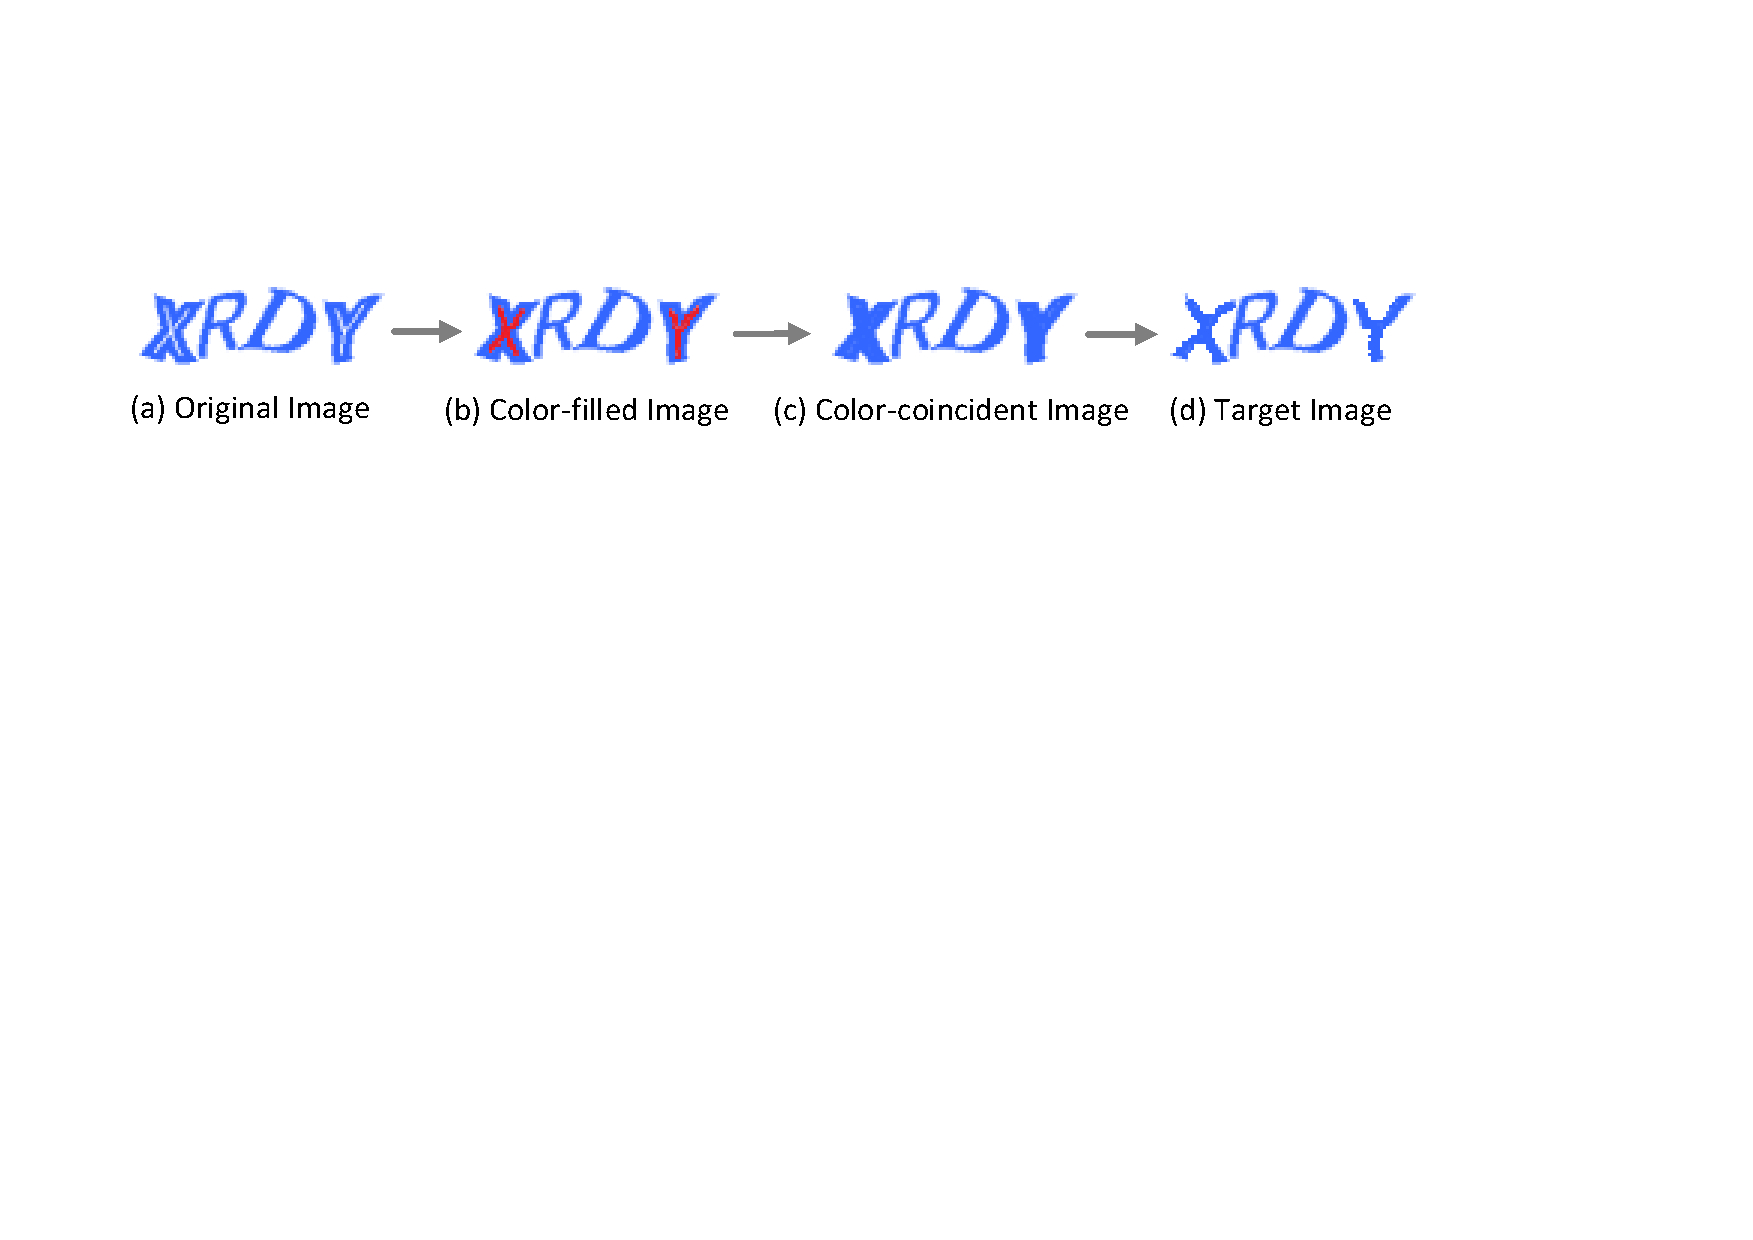
\includegraphics[width=0.5\textwidth]{fig/fill_color.pdf}
  \caption{The procedure of Captcha preprocessing.}
  \label{fig:fill_color}
\end{figure}

\noindent \textbf{\emph{Step 1. Captcha Preprocessing}}

The attack begins from inputting the distorted Captchas with complex background and overlapping characters. Given the characters on Captcha have different styles (see Figure~\ref{fig:fill_color} (a), it includes both hollow and solid characters), it is necessary to uniform the style of these characters for further processing. We have shown that the system can automatically translate the hollow character to the solid one (Figure~\ref{fig:fill_color}).

\noindent \textbf{\emph{Step 2. Generate Regular Captcha}}

Once the style of character on Captcha image is uniformed, a deep learning algorithm will be applied to generate the regular Captcha shown as Figure~\ref{fig:overview}. We archive this through hierarchical approaches described as the following three steps:

\noindent \circling{\textcolor{white}{1}} \textbf{Remove Noisy Background:}  To generate the regular Captcha, the first step is to clean the complex background, and produce the Captcha with white background.
To do so, a deep learning algorithm will be applied to remove the complex noisy background stay on Captcha.
For each Captcha scheme, this algorithm needs to train the model for cleaning out the background.

\noindent \circling{\textcolor{white}{2}} \textbf{Expand Space Between Adjacent Characters:} This step aims to increase the distance between two characters on Captcha. We use the same algorithm as step 2 to enlarge the inter-character distance and generate a new Captcha. Keep in mind that the Captcha generated at this stage is distorted.

\noindent \circling{\textcolor{white}{3}} \textbf{Regularization:} In this step, our system is able to automatically translate the distorted Captcha to a regular one.

\noindent \textbf{\emph{Step 3. Recognize Captcha}}

In this final step, we use a radical CNN model as the recognition engine to identify the text of the regular Captcha translated from last step.




%    \begin{algorithm}[!t]
        \centering
        \caption{Unifying the character font style}
        \label{alg:unify_font_style}
        \begin{algorithmic}[1]
            \REQUIRE~~\\
                $CI$: Captcha Image  \\
                $numChar$: The number of characters on Captchas\\
            \ENSURE~~\\
                $UC$: Captcha with the same font style \\
            \STATE $grayCI \leftarrow getBinaryImage(CI)$ \\
            \STATE $positions[] \leftarrow getHollowPositions(grayCI)$ \\
            \STATE $LEN \leftarrow getPositonsLen(positions[], numChar)$ \\
            \STATE $meanThick \leftarrow getMeanCharThick(CI, positions[])$ \\
            \FOR{$i=1:LEN$}
                \STATE $cFI \leftarrow FillRedColor(CI, positions[i])$ \\
                \STATE $cCI \leftarrow ChangeFillColor(cFI, positions[i])$ \\
                \STATE $charThick \leftarrow getCharThick(cCI, positions[i])$ \\
                \IF{$charThick>meanThick$}
                    \STATE $UC=cropChar(cCI, positions[i], meanThick)$ \\
                \ENDIF
            \ENDFOR
        \end{algorithmic}
    \end{algorithm}
\section{Implementation Details}

\subsection{Captcha Preprocessing}
Given some current text-based Captchas mainly consist of both solid character and hollow character (see Figure~\ref{fig:text-based captchas} (j) and (k)), the first step of our attack is to unify the different font styles to a fixed style. Here we aims to fill the hollow character with solid core due to the following two reasons:
(1) the hollow character can be easily transformed to the solid one but not the opposite.
(2) the solid character can be extracted more stable features than hollow character at the following step according to our preliminary experiments.

To do so, we first convert the colorful image to black-and-white using the standard threshold selection method proposed by Otsu~\cite{Ostu1979A}\footnote{Note that we only use the binarized image to locate the position of the hollow part of the character other than furthering processing.}.
Then the Color Filling Segmentation (CFS)~\cite{Yan2008A} is used to fill the hollow character with the red color (see Figure~\ref{fig:fill_color} (b)). Next, the color-filled image should be convert to color-coincident image by changing the red filled area to the original character color (see Figure~\ref{fig:fill_color} (c)). At last, the thick filled characters on the color-coincident image need to be cropped as the original character (see Figure~\ref{fig:fill_color} (d)).

Our method for unifying the character font style is described in Algorithm~\ref{alg:unify_font_style}.
The input to the algorithm is the original Captcha image with different font styles and the number of characters on this Captcha, and the output of the algorithm is the Captcha with solid characters. To locate the hollow characters, we first convert the colorful original image to binarized image (line 1). According to the binarized image, we can get the positions of the each hollow characters on the colorful Captcha image (line 2) because the size of colorful image is the same as the binarized image. For each hollow character, we use CFS method described above to fill it with red color (line 6) and then replace the red filled color with the character color to get the color-coincident image (line 7). Finally, we crop the filled character on the color-coincident image to unify the font style of characters (line 10).

\subsection{Generate Regular Captcha}
After unifying the character font style, we need to generate regular Captchas for better recognizing. We achieve this by employing an image-to-image translation algorithm called Pix2Pix~\cite{Pix2PixCode}. This algorithm automatically translate the image from the original style to the target style. In our case, the images to be translated are the Captchas with complex noisy background, overlapping and distorted characters (original style). These are supplied to the algorithm by a Captcha generator developed using a simple script (Section~\ref{section: Captcha_generator}). The algorithm tries to generate regular Captcha with appropriate character spacing and clean background (target style).

In order to generate regular Captcha, we propose the hierarchical methods that employ a variant approach of \emph{Pix2Pix} to complete the progressive tasks.
These hierarchical methods share the same methodology of the variant algorithm.
The main differences of these hierarchical approaches are the input and output images. The inputs of the first steps are the images with complex background, overlapping and distorted characters.
These inputting images are eliminated the complex background by the variant approach which outputs the Captcha images with white background, overlapping and distorted characters.
According to the outputs, the second step is to expand the space between the adjacent overlapping characters using the same variant method, and produces the Captcha images only with distorted characters.
Finally, the distorted characters are translated to the regular ones using the variant method.

\noindent \textbf{Hierarchical Methods.} The hierarchical methods are comprised of three sequenced models, and they can respectively achieve the tasks of removing complex background, expanding space between adjacent overlapping characters and translating the distorted Captcha to a regular one. The sequenced models share the same translation model.
The key part of the translation model is a variant of \emph{Pix2Pix}, which consists of a image generator and discriminator. They are competing with each other until reach Nash equilibrium when training processing (Section~\ref{section: GANs}).

In our case of removing background, the inputting data are the image pairs including the Captcha images with complex background and the images with white background.
The goal is to train a generative model that can translate the Captcha image with complex background to the images with white background.
During training, the image generator produces the fake image that similar to the image with white background by randomly add the noisy points to it. The fake image and the image with complex background compose an image pair.
For the composed image pair, the discriminator learns to classify between the real and fake pairs. This competing process will be terminated until the discriminator cannot classify the image pairs.
Unlike the \emph{Pix2Pix}, we use the L2 distance to figure out the loss of the generator as L2 loss can capturing the overall structure of the Captcha image, which contribute to removing the background.
\begin{equation}\label{equation: L2_loss}
    \mathcal{L}_{L2}(Gen) = \mathbb{E}_{x,y \epsilon C_{O}, z \epsilon N_{O}} \|y - Gen(x, z)\|_{2}
\end{equation}

Where $x$ is the Captcha image with white background, $y$ is the image with complex background and $z$ is the fake image with the noisy points.

\begin{figure}[!t]
  \centering
  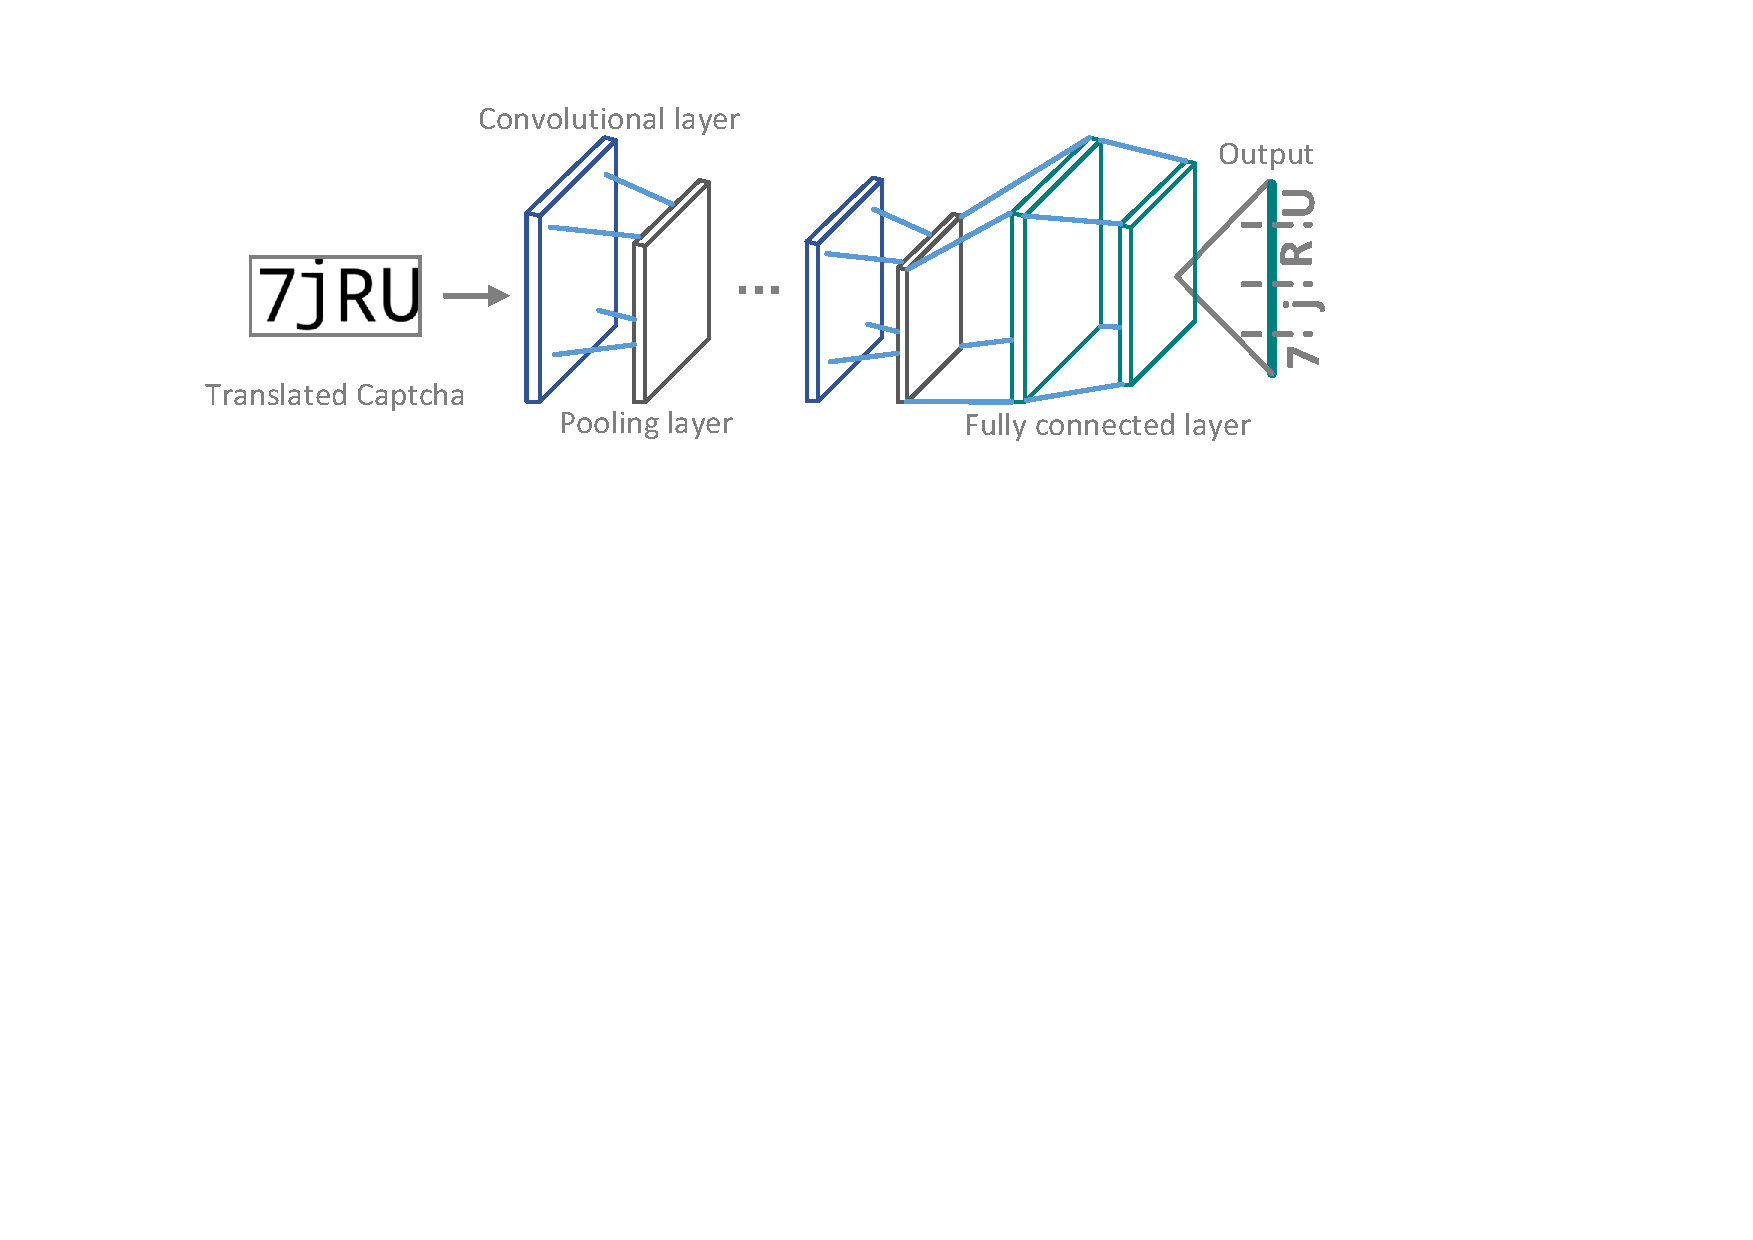
\includegraphics[width=0.45\textwidth]{fig/cnn_model.pdf}
  \caption{CNN recognition engine. The input of the recognition recognize is the regular Captcha image, and it output the text of the Captcha image.}
  \label{fig: cnn_model}
\end{figure}

\subsection{Identify Captcha}
In this step, we use a rudimentary CNN framework, \emph{LeNet-5}~\cite{Lecun1998Gradient}, as our recognition engine, to identify the text of the translated Captcha image.
The initial \emph{Lenet-5} was compromised of three convolutional layers, two pooling layers and followed by two fully connected layers.
The convolutional layer extracts the features using a number of filters that are trained during training process. The pooling layer aggregates the features extracted from the convolutional layer for extracting more representative features meanwhile reducing the amount of calculation. The fully connected layer classify the extracted features into target categories. The appropriate number of network layers determines the quality of the extracted features as proper number of layers will extract more representative features.

Unlike the \emph{LeNet-5}, the goal of our recognition engine is to recognize the text of Captchas on the whole, which is more difficult than recognition a single character done by \emph{LeNet-5}. This is because recognizing more characters need to extract more complex and abstract features.
To do so, we redesign the \emph{LeNet-5} and adding another two convolution layers and another three pooling layers.
Figure~\ref{fig: cnn_model} depicts the framework of our recognition engine. Generally, it consists of five convolution layers, five pooling layers and followed by two fully connected layers. Each convolution layer is followed by a pooling layer.

To extract more representative features, each convolutional layer uses a convolution filter of $3 \times 3$ and each pooling layer employs the max-pooling value. Other parameters are the same as the \emph{LeNet-5}.












%\input{material}
%\section{Related Work}
Our work lies at the intersection between adversarial machine learning and cracking text-based Captchas methods. This works brings together techniques developed in the domain of adversarial deep learning and character recognition to develop the attack on current text-based Captchas.

\noindent \textbf{Optical Character Recognition technology} Naor proposed the definition of Automated Turing Tests for automatically distinguishing humans from computer systems~\cite{Naor1996Verification}. This definition was firstly implemented by Lillibridge \emph{et al.}~\cite{Lillibridge2001Method} who developed the first practical scheme to prevent malicious bot programs from registering web accounts. However, such scheme was soon defeated by common used Optical Character Recognition (OCR) technique. Since then, a various of text-based and corresponding attacks have been proposed.

\noindent \textbf{Attacks on the individual Captchas} Mori~\emph{et al.}~\cite{Mori2003Recognizing} proposed an attack on Gimpy and EZ-Gimpy using complex object recognition algorithm. Their experiments shows that their approach can break 33\% Gimpy and 92\% EZ-Gimpy. Yan~\emph{et al.}~\cite{Yan2007Breaking} used a simple character segmentation method to break most Captchas provided by Captchaservices.org. They segmenting the character by counting the number of pixels of each individual character. Then they improved their character segmentation technique for attacking Microsoft-like Captcha schemes deployed by Yahoo!, Microsoft and Google~\cite{Yan2008A}. Gao~\emph{et al.}~\cite{Gao2013The} firstly proposed a generic method to break the hollow Captcha scheme. They first extracted the hollow character strokes based on color filling segmentation (CFS) method, and then searched for possible combinations of adjacent character strokes to form the individual characters. Recently they break Microsoft’s two-layer Captchas using similar approach with a high success rate~\cite{Gao2017Research}.
The above solutions first need to segment characters and then recognition them. But for the skewed and overlapped letters, their methods are hard to successfully segment as the characters are gathered together. To such scheme, Stark~\emph{et al.}~\cite{Stark2015CAPTCHA} presented an approach that can recognize the Captchas based on Active Deep Learning. Their approach can break Google's reCAPTCHA with a high success rate using a small number of labeled data.

\noindent \textbf{Generic attacks on text-based Captchas} Bursztein~\emph{et al.}~\cite{Bursztein2014The} reported a generic method to break a wide of text-based Captchas in a single step using machine learning algorithm. Their approach can recognize the Captcha by addressing the segmentation and recognition problems simultaneously. It scores all possible ways of character combinations to segment a captcha using reinforcement learning algorithm and search for the best possible one as the result.
More recently, Gao~\emph{et al.}~\cite{Gao2016A} present another generic approach that solved text-based Captchas. They first used Gabor filter to extract character components of the Captcha in four different directions, and then the extracted character components is ranked ordered by a graph search algorithm before recognizing the ranked components using Convolutional Neural Network.
The success of the two above approaches lies in the relative clean background. That is their approaches perfect poor when the Captcha has complex background as VISHOP scheme shown as Figure~\ref{fig:text-based captchas}. This is because their segmentation method cannot distinguish the individual character from such background.
George~\emph{et al.}~\cite{George2017A} proposed a novel network model named RCN that can break text-based Captchs using a samll number of training data.

\noindent \textbf{Study on the robustness of text-based Captchas} Bursztein~\cite{Bursztein2011Text} conducted a systematic study on existing text-based Captchas based on distorted characters. Among studying 15 Captcha deployed on popular websites, they found that 13 schemes excepting for Google and reCAPTCHA are vulnerable to automated attacks. They also explored whether it is easy to recognize the Captchas for human by conducting a large scale evaluation of Captchas from human's perspective~\cite{Bursztein2010How}. They collected 21 most widely used captcha schemes and asked the participants to manually recognize these Captchas. Their experiment results indicated that Captchas general were difficult for humans, especially for the audio Captcha schemes.
Krol~\emph{et al.}~\cite{Krol2016Better} carried out a user study on both reCAPTCHAs and "gamified" Captchas. They found that participants preferred to reCAPTCHAs than gamified Captchas because they were familiar with reCAPTCHAs.

\noindent \textbf{Attacks on other Captcha schemes} In addition to text-based Captchas, there are other Captchas such as image-based Captchas~\cite{Elson2007Asirra, Athanasopoulos2006Enhanced, Areyouhuman, Mohamed2017On, Gossweiler2009What}, audio-based Captchas~\cite{Schlaikjer2010A, Bigham2009Evaluating}.
However, researchers have proposed some attacks on image-based Captchas~\cite{Mohamed2014A, Gao2014An, Sivakorn2016I} and audio-based Captchas~\cite{Tam2008Breaking, Meutzner2014Reducing, Bursztein2009Decaptcha}, respectively. Further, such Captcha schemes are vulnerable to side-channel attacks~\cite{Hernandezcastro2009Side} as the limited number of example Captchas can be easily mined by the adversary.

\noindent \textbf{Adversarial machine learning} Recently, adversarial machine learning~\cite{Huang2011Adversarial} begins to be used in the field of information security. Researchers have found such technique can be used to evading classifiers of malicious software~\cite{Xu2016Automatically, Rosenberg2017Generic}, constructing specific malicious examples bypass intrusion detection system or spam e-mail filtering~\cite{Barreno2006Can} and cheat any classifiers trained by machine learning algorithms~\cite{Goodfellow2015Explaining, Miyato2015Distributional}.


%The Automated Turing Tests were first proposed by Naor~\cite{Naor1996Verification}, but they did not provide a formal definition. Lillibridge \emph{et al.}~\cite{Lillibridge2001Method} developed the first practical Automated Turing Test to prevent bots from automatically registering web pages. This system was effective for a while and then was defeated by common Optical Character Recognition (OCR) technology.
%
%Text-based Captchas based on English letters and Arabic numerals, is still the most widely deployed scheme. Many research communities focus on developing attack approaches for existing text-based Captchas, and then explore guidelines for better designs.
%
%A Captcha is considered broken if it can be automatically solved at a rate above 1\% at which Captchas are considered ineffective~\cite{Bursztein2011Text}. 

\section*{Acknowledgements}
    We would like to thank all participants who help for completing the experiments. Thank all volunteers for their time and insights as well as the anonymous reviewer for their critical and constructive comments. This work was supported by NSFC (Grant No. 61672427) and the UK Engineering and Physical Sciences Research Council (Grants No. EP/M01567X/1(SANDeRs) and EP/M015793/1(DIVIDEND)).

%\begin{spacing}{0.98}
\bibliographystyle{IEEEtranS}
\balance
\bibliography{refs}
%\end{spacing}

\end{document}
